\chapter{Introduction to flavour physics}
Ever since Democritus' philosophy of atomism, one of the driving desires behind mankind's advancements in the fields of natural science has been to reduce reality to its basic components. [...]

[...], this chapter explores the theoretical framework for the rest of thesis, introducing key concepts such as \textit{spin}, \textit{helicity} and the importance of \textit{angular distributions} of decay products.

\section{The Standard Model of Particle Physics}
[Introduzione? Da qualche parte devi definire la sigla SM.]

\subsection{Elementary particles}
\begin{figure}[t!]
	\centering
	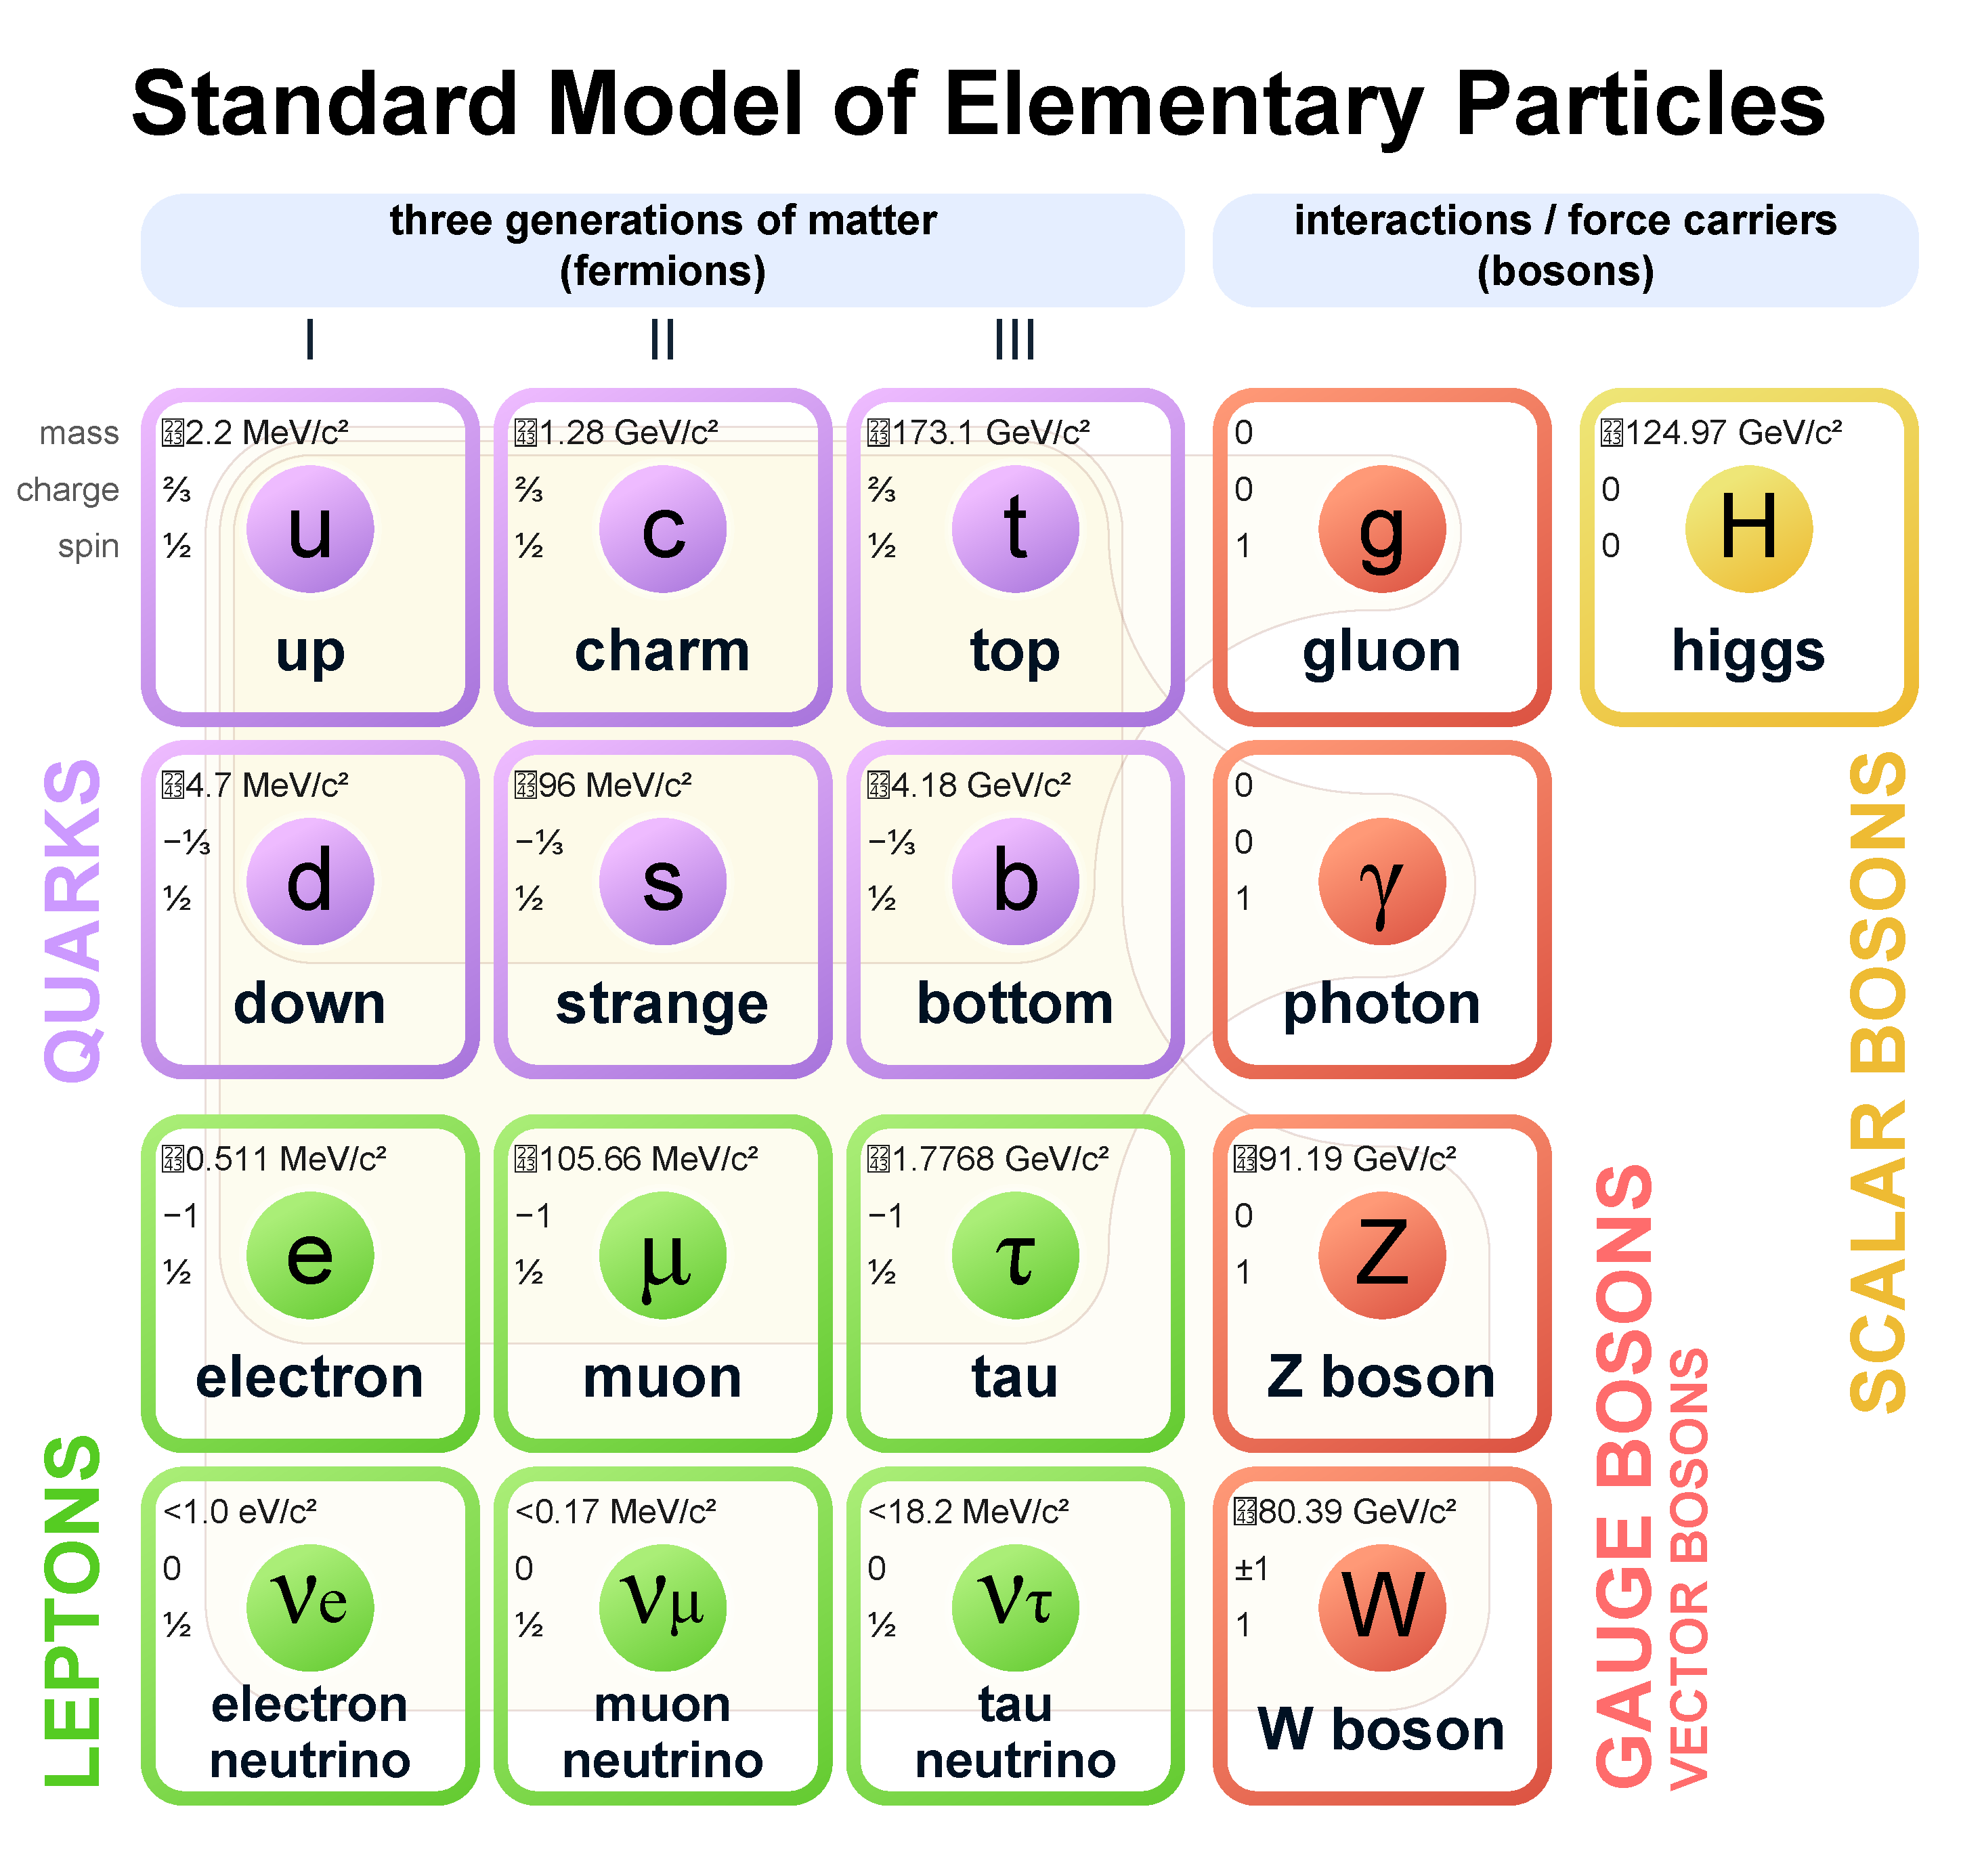
\includegraphics[scale=0.15]{graphics/01-standard_model/Standard_Model_of_Elementary_Particles.pdf}
	\caption[Currently known Standard Model elementary particles.]{The seventeen currently known elementary particles of the Standard Model. Antiparticles are not depicted.}
	\label{fig:particle_zoo}
\end{figure}

Intuitively, a particle is said to be \textit{elementary} when no substructure can be probed. 
A century of efforts in the fields of nuclear, quantum, and high energy physics has whittled down the spectrum of matter to just seventeen unique fundamental particles, colloquially known as the \textit{particle zoo} and depicted in Figure \ref{fig:particle_zoo}.

Each particle is joined by an \textit{antimatter particle} (\textit{antiparticle} for short), a companion of opposite charge identified by the prefix \textit{anti-}, e.g. antimuon for the muon; the only exception to this naming convention is the electron, whose antiparticle, for historical reasons, is known as positron.
While often omitted for the sake of brevity, antiparticles are elementary particles in every respect, distinct from their partners (bar the neutral gauge bosons, which are their own antiparticles) and related to them through the transformation of \textit{charge conjugation}.

\subsubsection{Leptons}
Leptons are fermions (half-integer spin particles) not sensitive to the strong nuclear interaction.
There are currently six \textit{flavours} of leptons grouped in three generations: each generation comprises a \textit{charged} lepton (electron, muon, tauon) and a \textit{neutral} lepton (electron neutrino, muon neutrino, tauon neutrino).

All charged leptons have a charge of $-q_e$, where $q_e$ is defined as the \textit{elementary positive charge}, and their mass ranges from $\approx \SI{0.5}{MeV}$ for the electron to over $\SI{1.7}{GeV}$ for the tauon.
By contrast, as the names suggest, all neutrinos are electrically neutral and are assumed massless in the Standard Model\footnote{The observation of flavour oscillation in solar neutrinos shows that neutrinos do in fact have non-zero, albeit very small, mass. This discrepancy is considered one of the major challenges to the Standard Model.}; this implies that their only meaningful interactions happen through the weak nuclear force, which grants them their characteristic evasiveness to most particle detectors.


\subsubsection{Quarks}
Much like leptons, quarks are also fermions existing in three generations. The main difference from the former category is that quarks, besides interacting through weak and electromagnetic forces, are also susceptible to the strong nuclear forces; this allows them to bind together in composite states known as \textit{hadrons}, which are classified as \textit{baryons} (states of three quarks) and \textit{mesons} (states of one quark and one antiquark).

Quarks can be classified as \textit{up-type} (up, charm and top quarks) and \textit{down-type} (down, strange and bottom quarks): up-type quarks have a fractionary charge of $+\frac{2}{3} q_e$, whereas down-type quarks have a charge of $-\frac{1}{3} q_e$. All quarks also have one of three \textit{color} charges (red, green or blue), while antiquarks similarly have one of three \textit{anti-color} charges (antired, antigreen or antiblue). A combination of all three colors/anti-colors or a combination of a color and its matching anticolor produces \textit{colorless} particles, a property of all observed quark composite states.

Unlike leptons, quarks are impossible to observe directly: according to the phenomenon of \textit{color confinement}, the energy of the interaction field between two color charges being pulled apart increases with their distance until it becomes high enough to create a quark-antiquark pair.
This process of \textit{fragmentation} develops many times over in such a way that the final observable state is entirely composed of colorless particles.
For this reason, high energy physics experiments such as LHCb do not detect free quarks, instead observing cone-shaped streams of hadrons known as \textit{hadronic jets}.

\subsubsection{Gauge bosons and fundamental interactions}
The fundamental forces driving the interactions between elementary particles are introduced in the Standard Model via the so-called \textit{gauge principle}.

[Gruppo di simmetria, principio di gauge, QCD e teoria elettrodebole.]

There is no gauge boson associated to the fourth known fundamental force, gravity.
Since every attempt to reconcile the general theory of relativity with quantum mechanics has failed so far, gravity is presently excluded from the Standard Model; this doesn't affect SM predictions at the subatomic level on account of the remarkably low intensity of said force, over 30 orders of magnitude lower than the weak interaction.

\subsubsection{The Higgs boson}
[Rottura spontanea della simmetria.]

\subsection{Flavour physics} \label{sec:flavour-physics}
A reader unfamiliar with SM terminology may find it amusing to employ the word \textit{flavour} to refer to what have been so far presented as different kinds of particles altogether.
However quirky, the lexical choice highlights a defining feature: flavour, much like the degree of sweetness in a recipe, can change.

As often happens in particle physics, the rules are somewhat easier for leptons. For a given generation $\ell = (e,\mu,\tau)$, one can define a \textit{lepton family number} $L_\ell$ as the difference between the number of particles and antiparticles of said generation, charged leptons and neutrinos alike:
\begin{equation}
L_\ell
\coloneqq
n(\ell^-) - n(\ell^+)
+
n(\nu_\ell) - n(\bar{\nu}_\ell).
\end{equation}
For all three generations, $L_\ell$ is conserved in every interaction except neutrino oscillations.

Quarks are not as straightforward.
A similarly defined quark flavour number, such as the so-called \textit{topness} (or \textit{truth})
\begin{equation}
T
\coloneqq
n(t) - n(\bar{t}),
\end{equation}
is preserved through EM and strong interactions, but can change when the state undergoes a \textit{weak charged interaction}, i.e. a weak interaction mediated by the charged gauge bosons $W^\pm$. In fact, one finds that weak interactions for quarks can be accurately described if we assume that the weak eigenstates $(d',s',b')$ of down-type quarks, i.e. the weak isospin doublet partners to up-type quarks, are related to the free mass eigenstates $(d,s,b)$ through a rotation:
\begin{equation}
	\begin{pmatrix}
		d' \\
		s' \\
		b'
	\end{pmatrix}
	=
	\begin{pmatrix}
		V_{ud} & V_{us} & V_{ub} \\
		V_{cd} & V_{cs} & V_{cb} \\
		V_{td} & V_{ts} & V_{tb}
	\end{pmatrix}
	\begin{pmatrix}
		d \\
		s \\
		b
	\end{pmatrix}.
	\label{eq:CKM_matrix}
\end{equation}
In this notation, the probability for a quark of flavour $i$ to change into a quark of flavour $j$ as a result of a weak charged interaction is proportional to ${\left| V_{ij} \right|}^2$.

The unitary rotation matrix is known as the Cabibbo-Kobayashi-Maskawa (CKM) matrix $V_\text{CKM}$.

[Valori numerici, riparametrizzazione con tre mixing angles e $\delta$ complessa.]

The complex phase $\delta$ is known as the CP-violating phase. To fully understand what it means and its role in particle physics, however, a digression into discrete symmetries is needed.

\section{Discrete symmetries and CP violation}
[Simmetrie in meccanica quantistica. Tre tipologie di simmetrie: continue, di campo e discrete. Sì, insomma, questa parte sono le lezioni di Giammarchi da riscaricarsi. Ops.]

\subsection{Parity}
[Descrizione, parità intrinseca, violazione e primo esperimento.]

\subsection{Charge conjugation}
[Descrizione, C-parità intrinseca, violazione e primo esperimento.]

\subsection{Time reversal}
[Descrizione, violazione e primo esperimento.]

\subsection{CP symmetry}
The sequential combination of C, P and T symmetries, commonly designated as CPT symmetry, plays a key role in the foundations of quantum physics.
As well as being the only combination of said symmetries still observed to be a symmetry of physical laws, the \textit{CPT theorem} states that any Lorentz-invariant local quantum field theory must be CPT-symmetric.
Because a violation of the CPT symmetry would imply the collapse of the modern quantum physics framework, it is generally accepted that a T-violating process must also be a CP-violating process.
This has an important consequence in the study of discrete symmetry violations: because of the of the self-evident hindrances in building a time-reversed experimental setup outside of trivial cases, every test of T violation becomes by necessity a test of CP violation.

[Esempio di soddisfazione di CP? Violazione della simmetria CP: osservazioni.]

The subject of CP violation is also closely tied to another long-standing dilemma in both particle physics and cosmology: the observed asymmetry between matter and antimatter in our Universe.
A perfectly CP-symmetric system would produce a roughly equal number of particles and antiparticles, which would annihilate each other and yield an empty Universe; our very existence implies a primordial imbalance that resulted in baryogenesis and therefore some degree of CP violation.

The observed asymmetry can be quantified through the \textit{baryon asymmetry parameter}, computed as the discrepancy between the densities of baryons and antibaryons normalized to the radiation density $n_\gamma$:
\begin{equation}
\eta \coloneqq \frac{n_B - n_{\bar{B}}}{n_\gamma}.
\end{equation}
Measurements from the cosmic microwave background
% ?
find $\eta_\textbf{CMB} \approx {10}^{-10}$, whereas the Standard Model predicts a much lower $\eta_\text{SM} \approx {10}^{-20}$.

New sources of CP violation are therefore required to match the observed value, with a promising field being the search for intrinsic electromagnetic dipole moments.

\section{Electromagnetic dipole moments}

[Anche se ho usato la parola con leggerezza nei capitoli precedenti], the concept of \textit{spin} may very well be one of the most challenging in particle physics.

\subsection{EDMs}

[Comportamento sotto CPT, evidenza che EDM non nullo implica violazione CP, mentre MDM può essere usato per testare CPT perché dev'essere uguale per particella-antiparticella.]

\subsection{MDMs}

\section{The \texorpdfstring{$\Lambda$}{Lambda} baryon}

Furthermore, unlike in the case of the prospective discovery of a neutron
EDM\footnote{Quantum chromodynamics (QCD), the theory describing the interaction of quarks and gluons, allows for a CP-violating term proportional to the QCD vacuum angle $\theta$. Current measurements of the neutron EDM constrain $\theta \lesssim {10}^{-10}$, a fine-tuning suppression known as the \textit{strong CP problem}; nevertheless, experimental discovery of a non-zero neutron EDM could be traced back to this term and would not necessarily require the introduction of new physics.},
a non-zero $\Lambda$ baryon EDM could not be explained by any phenomena within the Standard Model and would therefore imply the existence of BSM physics.

It can be shown (see Appendix \ref{chap:angular-distribution}) that the expected angular distribution for protons is...